\usetikzlibrary{shapes}
\usetikzlibrary{arrows}
\usetikzlibrary{calc,positioning}
\usetikzlibrary{automata} % LATEX and plain TEX
\begin{figure}[t]
\centering
\scalebox{0.9}{
	\scriptsize
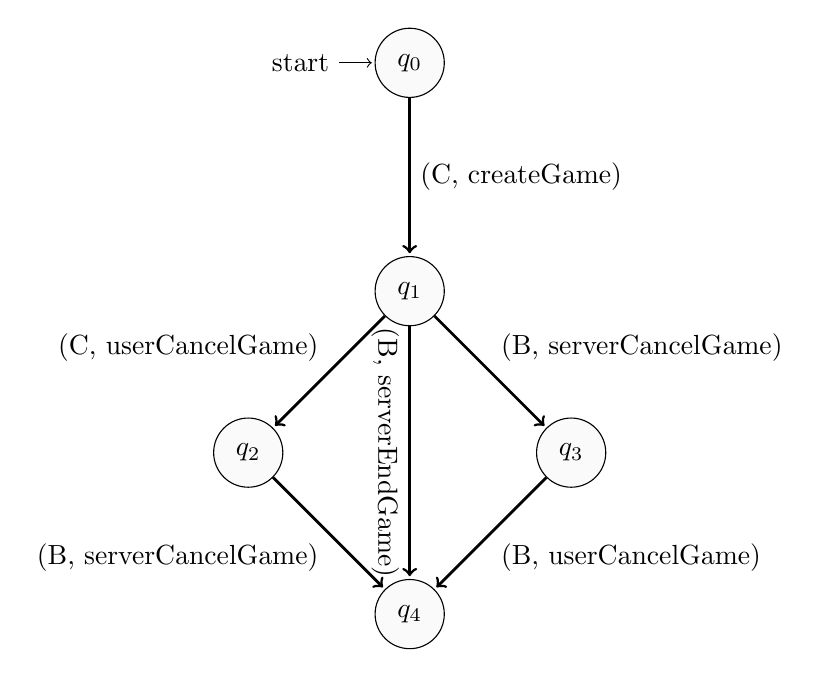
\begin{tikzpicture}[shorten >=1pt,node distance=2.9cm,auto]
	\tikzstyle{every state}=[fill={rgb:black,1;white,50}]
	\node[state,initial] (q0) {$q_0$};
	\node[state] (q1) [below of=q0] {$q_1$};
	\node[state] (q2) [below left of=q1] {$q_2$};
	\node[state] (q3) [below right of=q1] {$q_3$};
	\node[state] (q4) [below left of=q3] {$q_4$};
		
	\path[->, line width=1pt] (q0) edge node {(C, createGame)} (q1)
			  (q1) edge node [swap] {(C, userCancelGame)} (q2)
			  	   edge node {(B, serverCancelGame)} (q3)
	   			   edge node [below, rotate=-90] {(B, serverEndGame)} (q4)
	   		  (q2) edge node [below left] {(B, serverCancelGame)} (q4)   
	   		  (q3) edge node {(B, userCancelGame)} (q4)      
	   			   ;
			  
\end{tikzpicture}
}
\caption{The SFSM of Dicether.}
\label{fig: DicetherSFSM}
\end{figure}